\documentclass{article}
% Hyperreferences
\usepackage{hyperref}
% Margins
\usepackage[top=35mm,bottom=35mm,left=25mm,right=25mm]{geometry}
% Graphics and images
\usepackage{graphicx} \graphicspath{{./images/}}
\usepackage{subcaption}
\usepackage{float}
% Encodings (to render letters with diacritics and special characters)
\usepackage[utf8]{inputenc}
% Language
\usepackage[english]{babel}
% Section pagebreaks
\usepackage{titlesec}
\newcommand{\sectionbreak}{\clearpage}
\newcommand{\sectionnobreak}{% for when I want a section that does not break
  \global\toggletrue{afterpart}%
  \section
}
% Source code
\usepackage{listings}
\usepackage{xcolor}
\renewcommand{\lstlistingname}{File}
\lstset{
    frame=tb, % draw frame at top and bottom of the code
    tabsize=4, % tab space width
    numbers=left, % display line numbers on the left
	showstringspaces=false, % don't mark spaces in strings    
    commentstyle=\color{green}, % comment color
    keywordstyle=\color{blue}, % keyword color
    stringstyle=\color{red} % string color
}
\lstdefinelanguage{Maxima}{
	keywords={log,jacobian,determinant,subst},
	sensitive=true,
	comment=[n][\itshape]{/*}{*/}
}
% Tables with bold rows
\usepackage{tabularx}
\newcommand\setrow[1]{\gdef\rowmac{#1}#1\ignorespaces}
\newcommand\clearrow{\global\let\rowmac\relax}
\clearrow
% Math stuff
\usepackage[mathscr]{euscript}
\usepackage{amsmath,amssymb}
\usepackage{mathtools}
\usepackage{enumitem}
\newcommand{\expnumber}[2]{{#1}\mathrm{e}{#2}} % scientific notation
% Definitions, theorems, remarks,...
\usepackage{amsthm}
\newtheorem{definition}{Definition}[section]
\newtheorem{theorem}{Theorem}[section]
\newtheorem{corollary}{Corollary}[theorem]
\newtheorem{lemma}[theorem]{Lemma}
\renewcommand\qedsymbol{$\blacksquare$}
\theoremstyle{remark}
\newtheorem*{remark}{Remark}
% Contents title
\addto\captionsenglish{\renewcommand*\contentsname{Table of contents}}
% Headers and footers
\usepackage{fancyhdr}
\pagestyle{fancyplain}
\fancyhf{}
\lhead{ \fancyplain{}{LabWars - Final report (LCOM 2019/20)}}
\lfoot{ \fancyplain{}{T5G03}}
\rfoot{ \fancyplain{}{\thepage} }
%
\newcommand{\email}[1]{
{\texttt{\href{mailto:#1}{#1}} }
}
\newcommand{\role}[1]{
\begin{tabular}{l l}
	\begin{minipage}[t]{30mm} \textbf{Roles} \end{minipage} &
	\begin{minipage}[t]{125mm} #1 \end{minipage}
\end{tabular}\\
}
\newcommand{\func}[1]{
\begin{tabular}{l l}
	\begin{minipage}[t]{30mm} \textbf{Functionalities} \end{minipage} &
	\begin{minipage}[t]{125mm} #1 \end{minipage}
\end{tabular}\\
}
% Metadata
\title{\Huge LabWars \\ \Large Final report \\ \vspace*{4pt} \large LCOM 2019/20}
\author{
T5G03\\
\begin{tabular}{r l}
	\email{up201806429@fe.up.pt} & Diogo Miguel Ferreira Rodrigues        \\
	\email{up201806554@fe.up.pt} & Telmo Alexandre Espirito Santo Baptista
\end{tabular}
}
\date{06/01/2020}
% Document
\begin{document}
%\begingroup
	\maketitle
%	\let\clearpage\relax
%	\setcounter{tocdepth}{2}
	\tableofcontents
%\endgroup
\section{User instructions}
\subsection{How to play}
In all game modes, the controls are the same:
\begin{itemize}
	\item \textbf{WASD} to move North, East, South and West respectively.
	\item \textbf{Mouse left-click} to fire a bullet.
	\item \textbf{Ctrl+'+'} and \textbf{Ctrl+'-'} to zoom in and out.
	\item \textbf{ESC} to escape game mode (go back).
\end{itemize}
\subsection{Main menu}
On startup, users are greeted by a \texttt{Loading...} message, briefly followed by the main screen.
\begin{figure}[H] \centering
	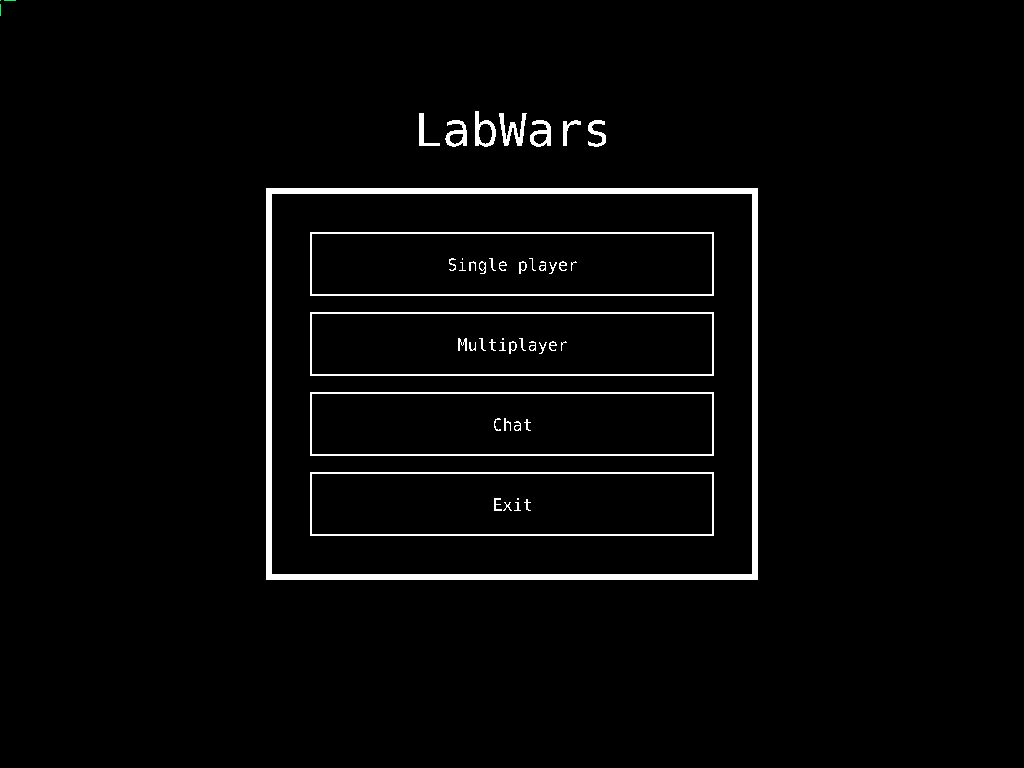
\includegraphics[scale=0.45]{main_menu}
	\caption{Main menu}
\end{figure}
Using the mouse movement and clicks, the user can select one of the avaliable options:
\begin{itemize}
	\item \textbf{Single player}: Go to single player selection menu, to select one of the single player game modes.
	\item \textbf{Multiplayer}: Go to multiplayer mode, allowing to select more options.
	\item \textbf{Chat}: Exchange text messages with another connected computer.
	\item \textbf{Exit}: Exit the game
\end{itemize}
The user can also exit the game by presing \textbf{ESC}.
\pagebreak
\subsection{Single player}
Upon entering into single player mode, the user is presented with a menu from which he can choose one of the options. \par
\begin{figure}[H] \centering
	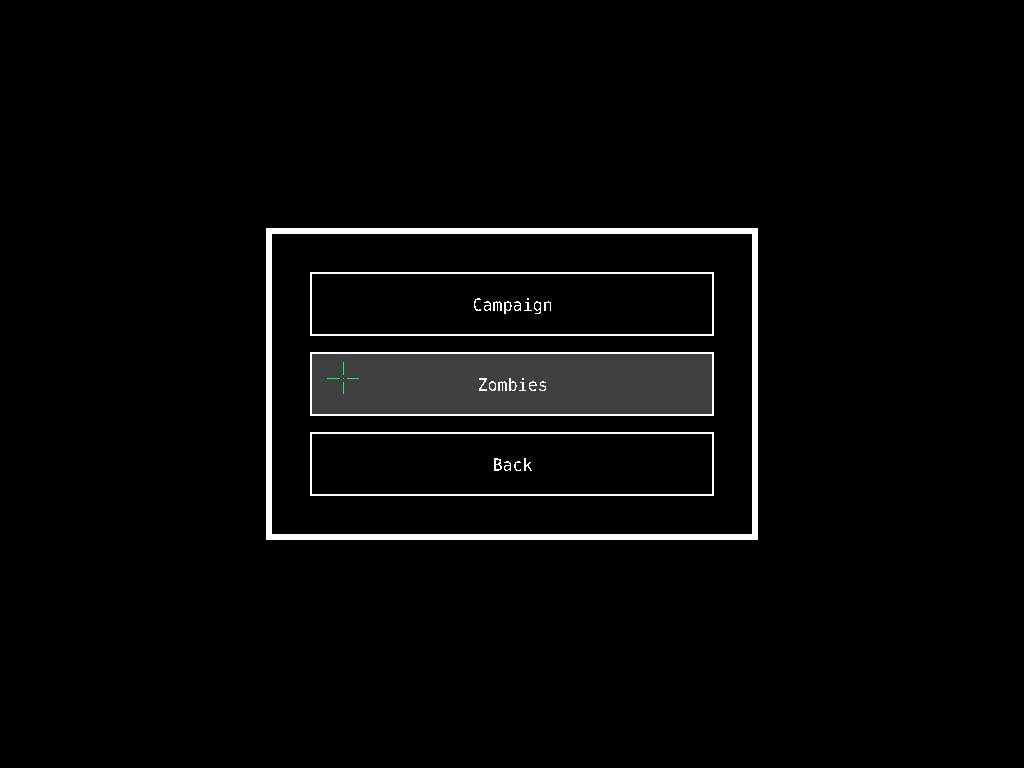
\includegraphics[scale=0.45]{singleplayer01}
	\caption{Single player menu}
\end{figure}
\begin{itemize}
	\item \textbf{Campaign}: campaign mode; kill all autonomous opponents.
	\item \textbf{Zombies}: zombies mode; kill as many zombies and survive as much time as possible.
	\item \textbf{Back}: go back to main menu.
\end{itemize}
The user can also go back to main menu by pressing \textbf{ESC}.
\pagebreak
\subsubsection{Campaign}
In campaign mode the goal is to kill all the opponents in the map as fast as possible, while sustaining as little damage as possible.
\begin{figure}[H] \centering
	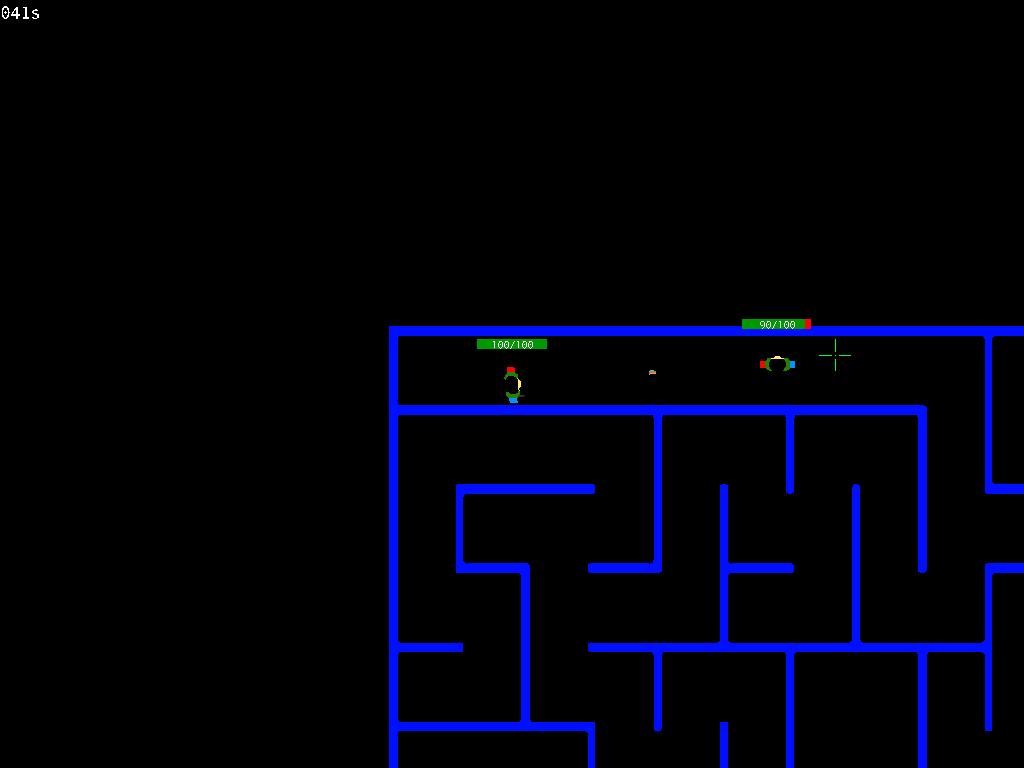
\includegraphics[scale=0.45]{campaign01}
	\caption{Campaign mode}
\end{figure}
\pagebreak
\subsubsection{Zombies}
In zombie mode the goal is to kill as many zombies and survive as much time as possible. Zombies slowly follow the player and attack the player when in short range.\par
Once the player kills a zombie, a new zombie spawns in a random part of the map, with more life than all previous zombies.
\begin{figure}[H] \centering
	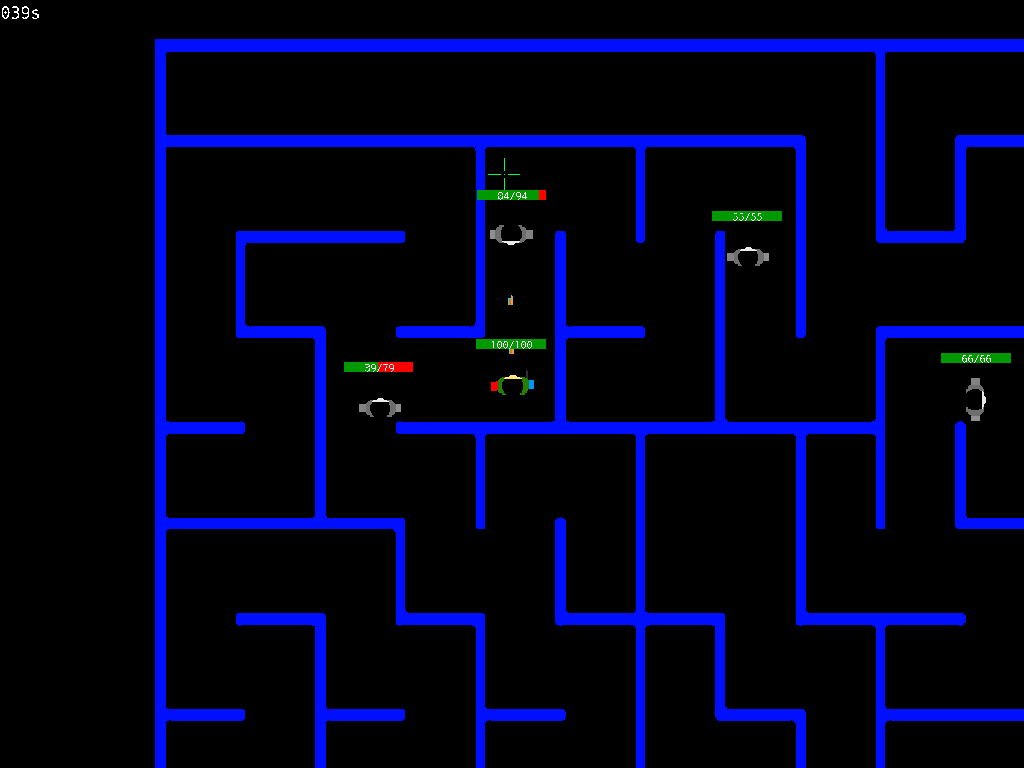
\includegraphics[scale=0.45]{zombies01}
	\caption{Zombies mode}
\end{figure}
\pagebreak
\subsection{Multiplayer}
In multiplayer mode, 
\pagebreak
\subsection{Chat}
This chat tool was initially designed as a simple, text mode, test communication between different machines. We have however decided to include it as a functionality in the project for a number of reasons:
\begin{enumerate}
	\item It was easy to develop the graphical part and integrate in the project.
	\item Having a friendly functionality that uses the communication modules allows for faster debugging; in case the computers are not properly connected, or if during development something stops working we can immediately check if the communication modules also stopped working.
	\item It served as a minimal insurance that our project would integrate the communication modules, in case we could not implement multiplayer mode.
	\item It is a useful feature.
\end{enumerate}
\begin{figure}[H] \centering
	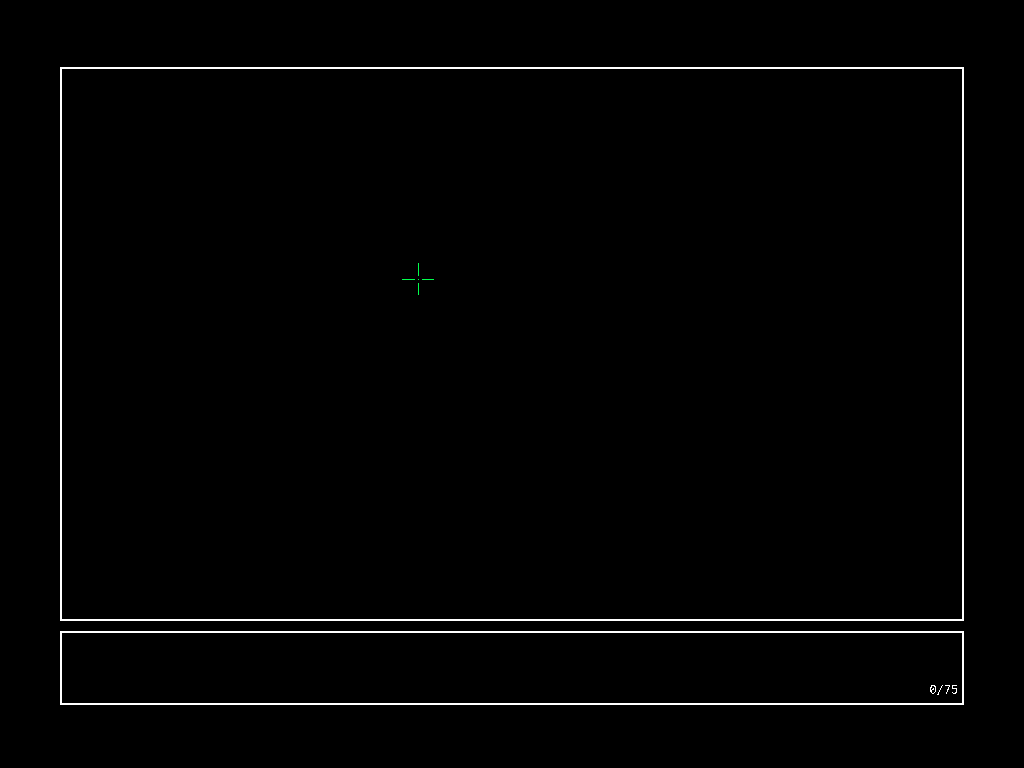
\includegraphics[scale=0.45]{chat01}
	\caption{Chat environment}
\end{figure}
The chat can be used for exchanging messages of up to 75 characters directy writable with the keyboard. The character limit was imposed to prevent strings from rendering as wider than the input box, and the fact they should be directy writable with the keyboard simplifies the process of capturing scancodes, having as downside not allowing to write characters that require more than one key press (like exclamation or question marks in a Portuguese keyboard). \par
\begin{figure}[H] \centering
	\begin{subfigure}[b]{0.48\linewidth}
		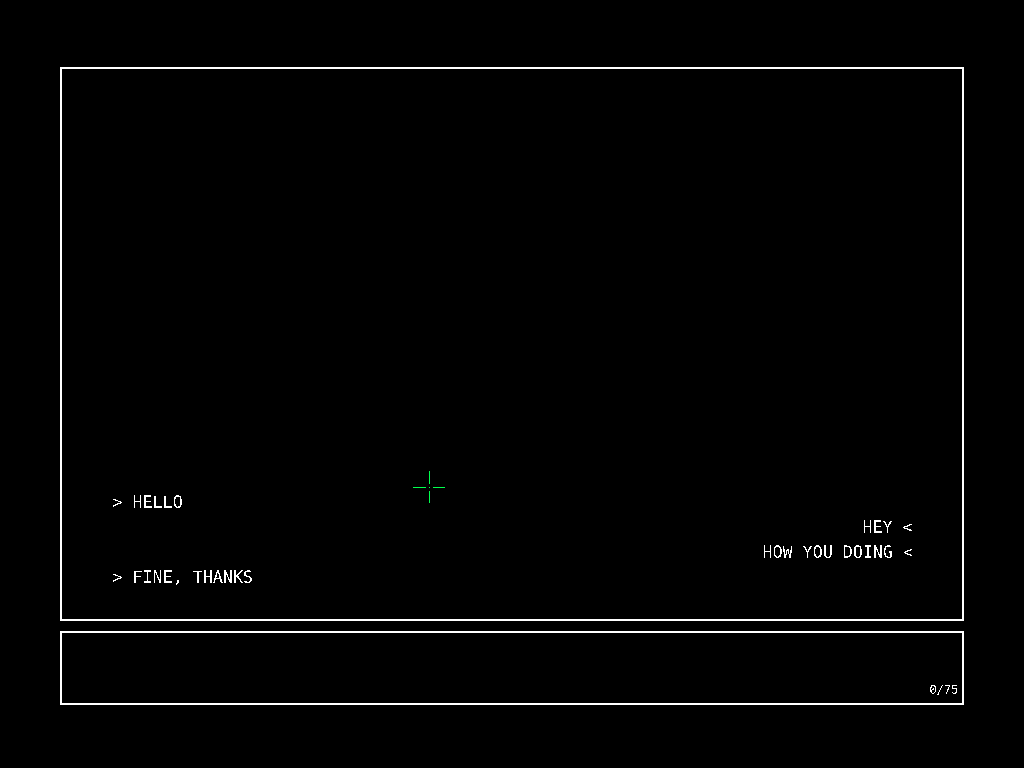
\includegraphics[width=\linewidth]{chat02_01}
		\caption{Computer 1 chat}
	\end{subfigure}
	\begin{subfigure}[b]{0.48\linewidth}
		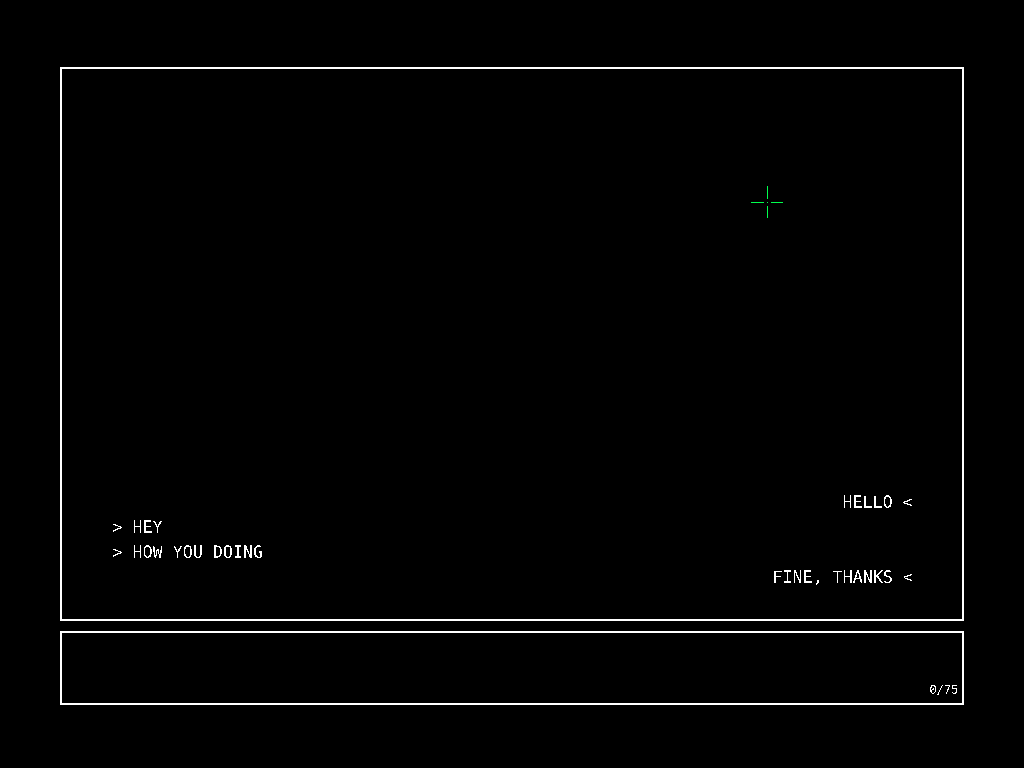
\includegraphics[width=\linewidth]{chat02_02}
		\caption{Computer 2 chat}
	\end{subfigure}
	\caption{Two users interacting via chat}
\end{figure}
The user can exit the chat mode by pressing \textbf{ESC}.
\section{Project status}
All functionalities previously presented were fully implemented, with the exception of:
\begin{itemize}
	\item \textbf{Campaign}: autonomous opponents were supposed to follow a pre-programmed path and shoot on sight at the player. Currently, they don't do either of those.
	\item \textbf{Multiplayer}: still working on it.
\end{itemize}
The I/O devices used in the project are presented in the following table.
\begin{center} \begin{tabular}{c || l | c}
	\textbf{Device} & \textbf{What for}                                        & Method \\ \hline
	Timer           & Frame rate, time since beginning of game                 & Interrupts \\
	Keyboard        & Player movement, writing chat messages                   & Interrupts \\
	Mouse           & Player orientation, shooting, selecting options in menus & Interrupts \\
	Video card      & In-game drawing, menus                                   & None \\
	RTC             & Scoreboards                                              & Polling \\
	Serial port     & Chat communication, multiplayer modes                    & Interrupts
\end{tabular} \end{center}
To manage all interrupt subscriptions, the general function \texttt{unsubscribe\_interrupt} was implemented and used.
\subsection{Timer}
Timer 0 is used to generate periodic interrupts at a rate of 60Hz, essentially controlling a large part of what the program does.\par
Timer interrupts regulate screen refreshing, which happens at a rate of 60Hz. In all game modes, timer interrupts serve not only the purpose of refreshing the screen, but also to process all the game data: collisions, movement, path-finding algorithms, etc. \par
To manage timer interrupt subscriptions, functions \texttt{subscribe\_timer\_interrupt}, \texttt{timer\_int\_handler} and \texttt{timer\_get\_no\_interrupts} were implemented and used.
\subsection{Keyboard}
The keyboard was configured to issue interrupts on key presses and releases.

To manage keyboard interrupt subscription, function \texttt{subscribe\_kbc\_interrupt, } was implemented. To manage keyboard interrupts, functions \texttt{kbc\_ih}, \texttt{keyboard\_get\_scancode} were implemented and used. 

\func{Keyboard in interrupt mode.}
\subsection{Mouse}
\func{Mouse buttons and movement in interrupt mode.}
\subsection{Video card}
\func{Video Card in graphic mode with direct color encoding, dynamic updating of VRAM/screen.}
\subsection{Real-Time Clock (RTC)}
\func{Use of the RTC functionalities needed to implement the requirements stated in the role of the device.}
\subsection{Serial port}
\func{Point-to-point communication between two computers.}
\pagebreak
\section{Code organization/structure}
Hey
\section{Implementation details}
Hey
\section{Conclusions}
Hey
\end{document}
